%!TEX root = ../thesis.tex
%*******************************************************************************
%******************************   Fourth Chapter   ***************************
%*******************************************************************************
\chapter{Improving \ont{} sequencing accuracy for \mtb{}}
\label{chap:tubby}
%%%%%%%%%%%%%%%%%%%%%%%%%%%%%%%%%%%%%%%%%%%%%%%%%%%%%%%%%%%%%%%%%%%%%%%%%%%%%%%%%
\begin{markdown}


### An \mtb{} species-specific \ont{} basecalling model improves accuracy

It has previously been shown(CITE) that a taxon-specific basecalling model can improve both the read-level and consensus accuracy of \ont{} sequencing reads. While this was shown for *Klebsiella pneumoniae*, it remains to be seen if this approach generalises to other species. The major difficulty in producing such a model pertains to the requirement for a "truth" genome for the training data. The \ont{} basecaller, \guppy{}, uses neural networks to convert raw signal into a DNA sequence. In order to train the network in how to make this inference it is necessary to label the raw signal with its corresponding "truth" sequence. Such datasets are difficult to find for certain species. However, the dataset we have collected for the work in this chapter is perfectly suited as we have reads from Illumina, PacBio, and \ont{} that are from the *exact* sample DNA extraction. As the bulk of the work in this chapter (and the subsequent chapters) has an implicit reliance on the quality of the \ont{} basecalling accuracy, we sought to train a \mtb{}-specific \guppy{} model.  

To facilitate the training of the \mtb{}-specific model we used the \ont{} model-training tool \taiyaki{} (see \todo{add link to relevant methods section}). We use the samples with matched PacBio data for the training as they have high quality assemblies that can be used as truth (\autoref{sec:asm_results}). With the aid of \taiyaki{} we map the basecalled \ont{} reads to the truth assembly; creating a truth sequence for each read. The truth sequence for each read is then mapped to the raw signal, which is the main input format for training. Across the eight samples there was a total of 1,309,049 \ont{} reads that were mapped. Reads were split into training (20\% - 261,808 reads) and evaluation (80\% - 1,047,241 reads) sets. The model was trained by \taiyaki{} (using only the training set) and took 108 hours (4.5 days) to complete on 2 GPUs. The resulting \mtb{} model (referred to as 'tubby') was then used to re-basecall the reads in the evaluation set. We evaluate the tubby model and the default \guppy{} model inline with Wick *et al.*(CITE)(see \todo{add link to relevant methods section}).

#### Read BLAST identity

The first evaluation metric, read BLAST identity, determines the read-level accuracy produced by the basecalling model. We align the basecalled reads to the truth assembly and calculate BLAST identity as, for each mapping, the number of matching bases divided by the length of the alignment. \autoref{fig:combined_basecall}A shows the tubby model has a higher read-level BLAST identity (median 0.941) than \guppy{} (median 0.920).

#### Relative read length

We define relative read length as the length of the aligned part of the read, divided by the total length of the read. The purpose of this metric is to see whether there is a bias towards insertions (greater than 1.0) or deletions (less than 1.0). \autoref{fig:combined_basecall}C shows that, at the read level, tubby has a slight tendency towards deletions (shorter reads) compared to \guppy{} with median relative read lengths of 0.982 and 0.993 respectively. However, this result is a little more complex than just looking at median values. The distribution of lengths for \guppy{} extends much further past 1.0 compared with tubby, indicating an increase in insertions. We will return to this result when we look at the error types.

#### Consensus accuracy

To assess consensus accuracy the basecalled reads were assembled using `rebaler`. `rebaler` was developed by Wick *et al.* for the purposes of evaluating basecalling models and is a reference-guided assembly approach (see \todo{link to relevant methods section}). Here we show consensus accuracy in a similar manner to read identity. Each "read" in this context is the result of chopping the `rebaler` assembly of the reads up into 10kbp "chunks" to simulate reads. These chunks are then mapped back to the original assembly and we use BLAST identity as the measure of accuracy. \autoref{fig:combined_basecall}B shows tubby has higher consensus accuracy (median 0.9993) compared with \guppy{} (median 0.9992). The consensus accuracy improvement of 0.0001 equates to approximately 440 less erroneous positions in the \mtb{} assembly.

\end{markdown}

\begin{figure}
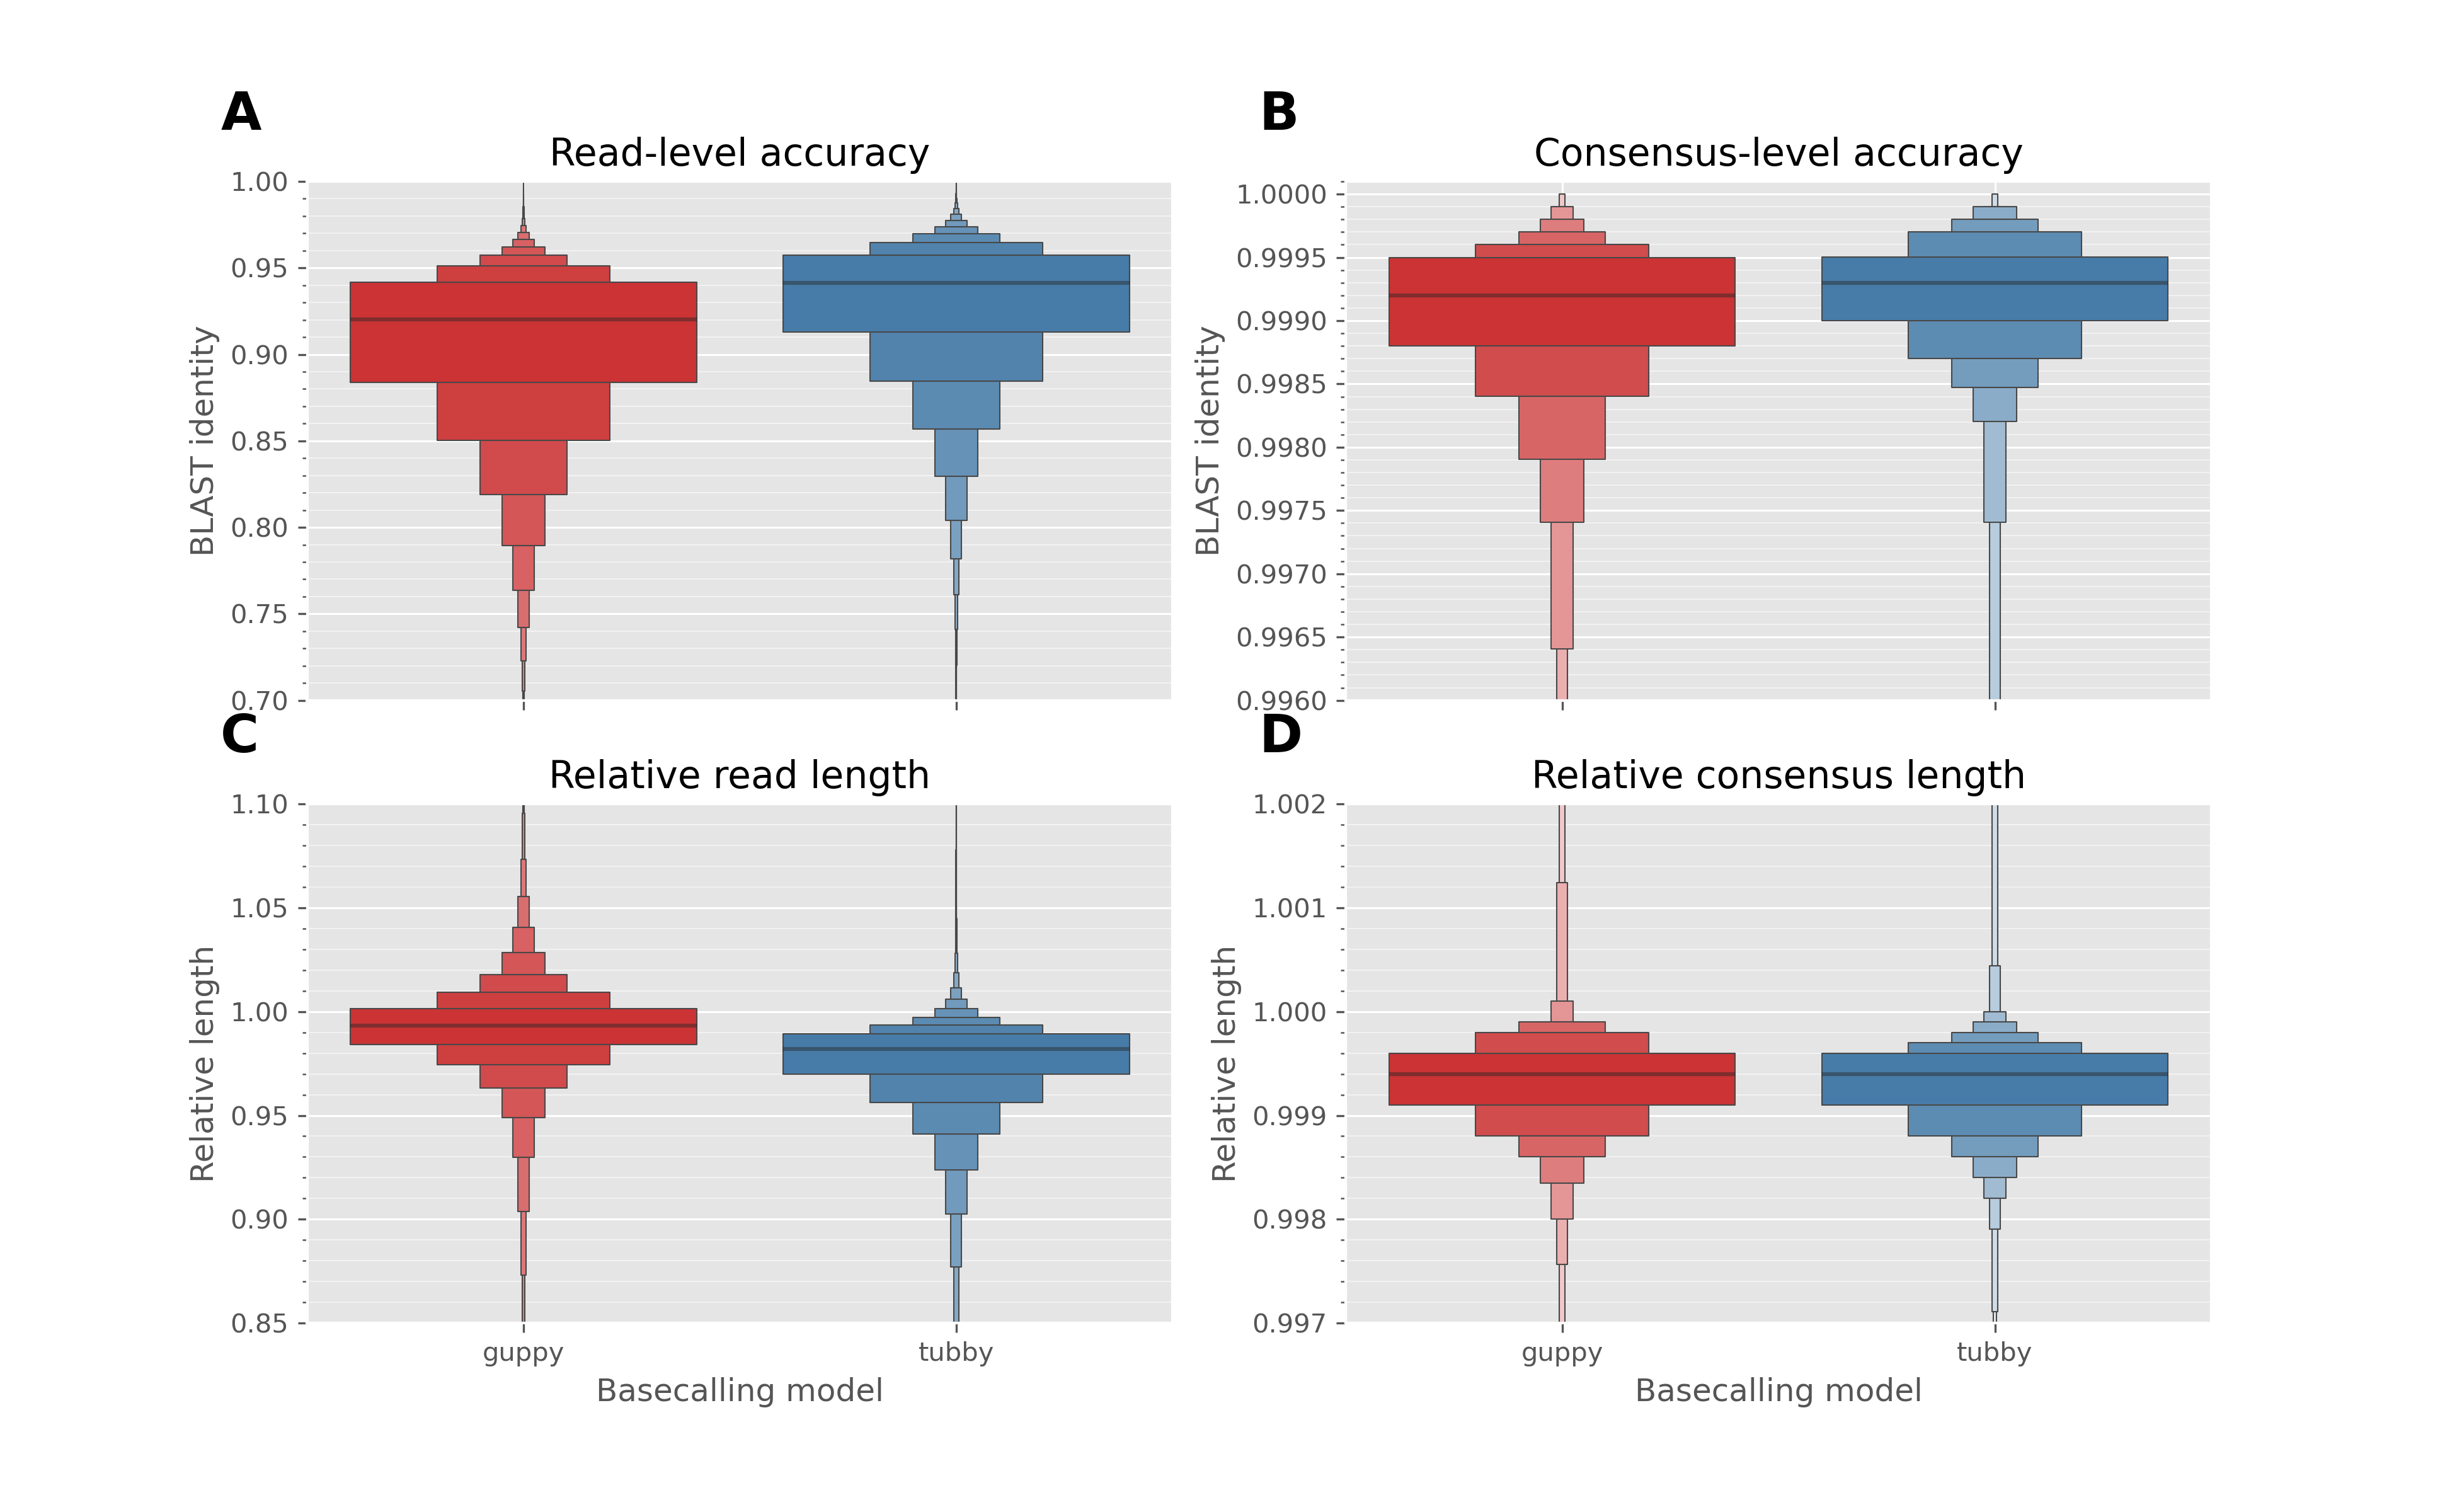
\includegraphics[width=1.0\textwidth]{Chapter4/Figs/combined_identity_relative_len.png}
\centering
\caption{A) Read BLAST identity (Y-axis) for the \mtb{}-specific basecalling model 'tubby' (blue) compared with the default \guppy{} model (red). BLAST identity is the number of matching bases (in a read alignment) divided by the length of the alignment. B) Consensus BLAST identity (Y-axis), where consensus refers to "chunks" of the genome assembly produced by the basecalled reads, for each model, mapped to the truth genome. C) Relative read length (Y-axis) for the two models. Relative read length is the length of the aligned part of the read, divided by the total length of the read. D) Consensus relative length. Relative length is the length of the aligned part of the consensus "chunk", divided by the total length of the "chunk". Note: the Y-axes have all been zoomed-in to allow closer inspection of the majority of data.}
\label{fig:combined_basecall}
\end{figure}

\begin{markdown}

#### Error types

Here we classify the types of errors that occur in the `rebaler` assemblies and look at how these errors compare across models. To determine the errors, we categorise the differences between the truth and `rebaler` assemblies (see \todo{link to relevant methods}). \autoref{fig:error_types} shows that the greater part of the error types (for both models) are attributable to deletions, with most being homopolymer deletions. We do however see that, except for non-homopolymer deletions, tubby's errors are lower than \guppy{}'s \todo{add some concrete numbers}. In the case of both insertion types, tubby has approximately 3.5-fold less insertions than \guppy{} - although these constitute a small portion of the overall errors. Both models have a very low level of Dcm-methylation errors, which is a nice control of sorts as \mtb{} does not have any known 5-methylcystosine methyltransferases(CITE)\improvement{ensure the wording of this and correct and that the claim is also correct}.

\end{markdown}

\begin{figure}
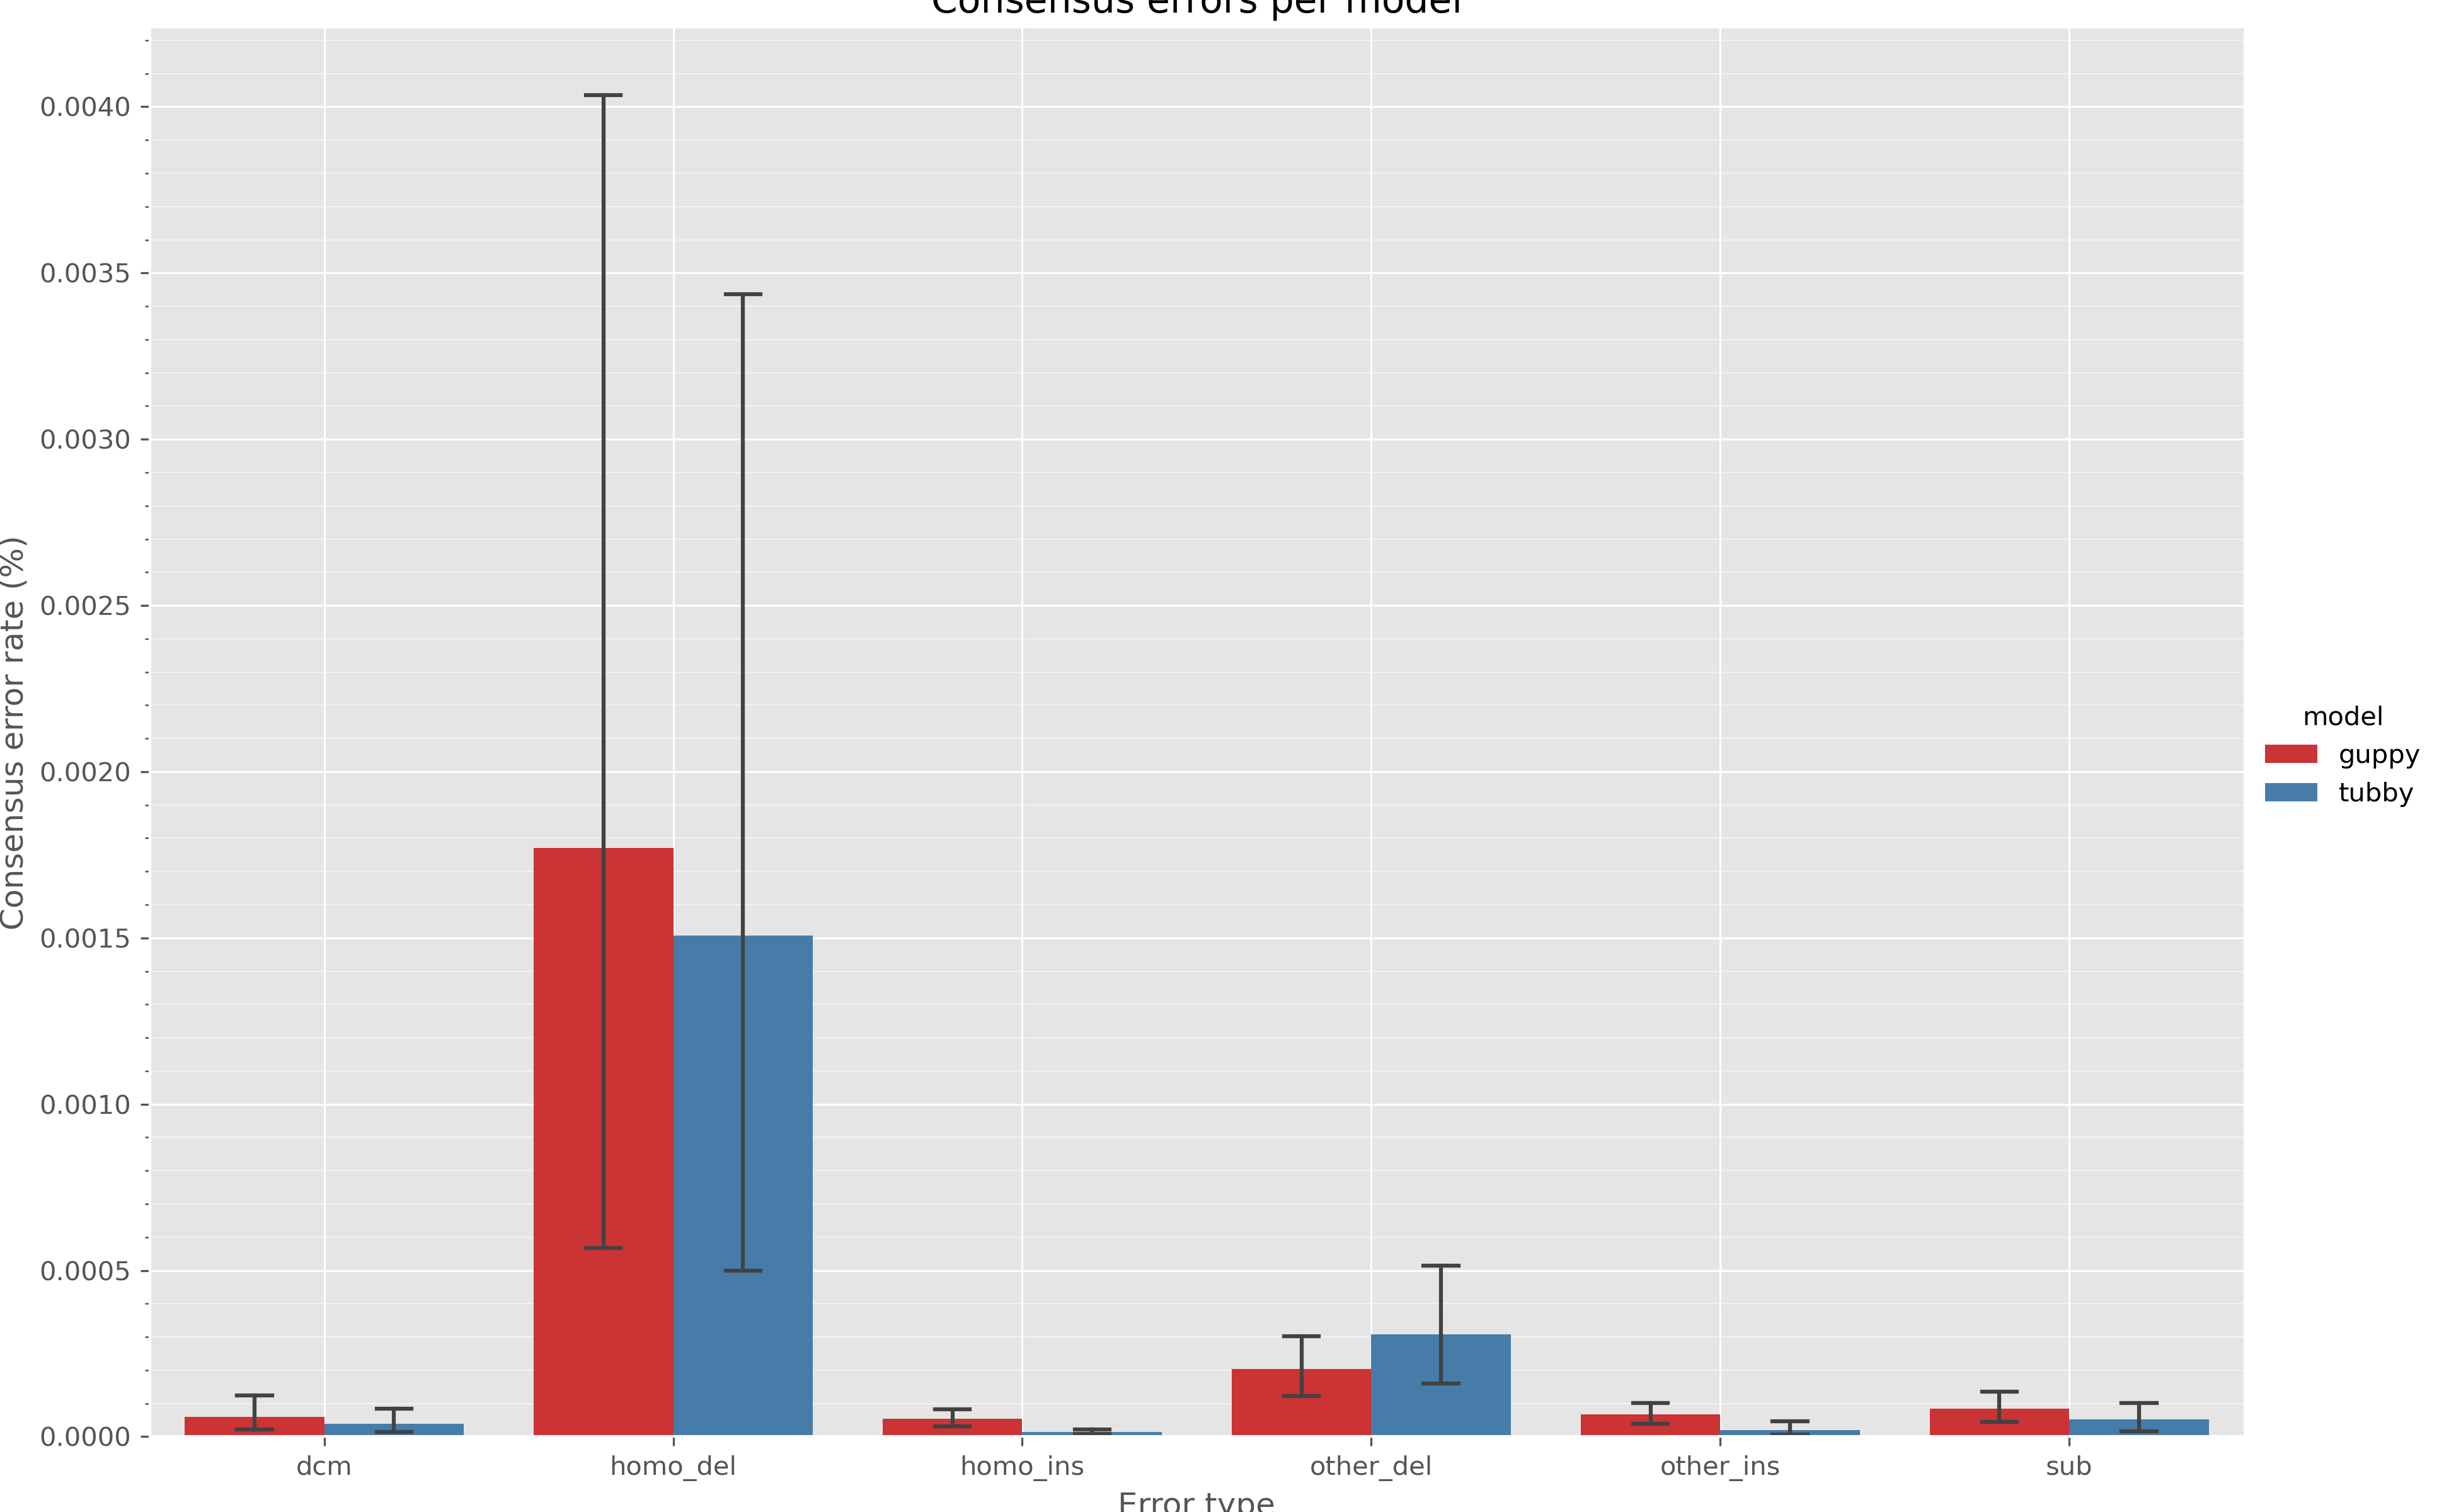
\includegraphics[width=1.0\textwidth]{Chapter4/Figs/consensus-error-types.png}
\centering
\caption{Error types in the `rebaler` assemblies produced from reads basecalled with tubby (blue) and \guppy{} (red). The consensus error rate is the percentage of the assembly these errors compose. The errors are per-assembly, so the confidence intervals represent variation in error types between samples/assemblies. dcm refers to Dcm-methylation motifs. homo\_ins/del are homopolymer insertions or deletions. sub is single-base substitutions.}
\label{fig:error_types}
\end{figure}

\begin{markdown}

\\

Given the improved performance across nearly all metrics for a \mtb{}-specific \ont{} basecalling model, tubby will be used for the remainder of this work. 


%%%%%%%%%%%%%%%%%%%%%%%%%%%%%%%%%%%%%%%%%%%%%%%%%%%%%%%%%%%%%%%%%%%%%%%%%%%%%%%%%

### Training a \mtb{}-specific \ont{} basecalling model

Taxon-specific \ont{} basecalling models have been shown to provide increased read and consensus accuracy(CITE). One of the most challenging aspects of training such a model though, is providing a truth sequence for the \ont{} data. Ideally, the training data should be from the same DNA extraction as the sequencing reads that produced the truth sequene. This ensures any discrepancies between the \ont{} data and the truth as technology differences, and not *in vitro* evolution. Given we have sequencing reads from the same DNA extraction across three sequencing technologies for nine samples, we chose to train an \mtb{}-specific model using the highest quality PacBio assembly from (\todo{link to asm methods}) for each sample as the truth. Using the PacBio assembly ensures no systematic biases from the \ont{} data are being reinforced.   
After assessing the final assemblies \todo{link to asm results}, we excluded sample one sample (`mada_1-2`) as it was found to contain three species and even after filtering out the contaminating contigs, the \mtb{} sequence was deemed too low quality for a truth assembly.  
\ont{} provides a software suite, \taiyaki{}(CITE), to prepare data for and perform model training. The first step in training the model is mapping the \ont{} basecalled reads to the respective truth sequence for each sample. The mapping is done using `minimap2`(CITE), and we use parameters that ensure it only outputs primary alignments. The sequence for each read is then replaced with the reference sequence it aligns to and written out to a Fasta file using a \taiyaki{} script. The eight "read-reference" Fasta files are then combined into a single file. The recommended number of reads for model-training is somewhere in the range of tens-of-thousands or low hundreds-of-thousands if lengths are greater than 1000bp or less than 500bp, respectively, on average (personal correspondence with \ont{} staff). The resulting aggregated read-reference Fasta file contained 1,309,759 entries. As this is far more sequences than is required, we randomly sub-sampled the Fasta file into two chunks with 20\% (261,950) for training and the remainder (1,047,807) to be used for validation of the final model. Using the list of read identifiers in these two subsets, we additionally subset the raw data, used for training, for each read into separate locations for training and evaluation. A script from \taiyaki{} is then used to align the raw signal for a read to its sequence in the read-reference file. This mapping is a vital preparation step that indicates what nucleotides are the result of a given collection of the raw signal. The raw signal mapping file was then passed to the model-training script from \taiyaki{} and training took 108 hours (4.5 days) to complete on 2 GPUs.

%%%%%%%%%%%%%%%%%%%%%%%%%%%%%%%%%%%%%%%%%%%%%%%%%%%%%%%%%%%%%%%%%%%%%%%%%%%%%%%%%

### Evaluating a custom \ont{} basecalling model

The model-training process produces a JSON file that can be used to basecall \ont{} reads with \guppy{}. The first step in evaluating whether our \mtb{}-specific model, 'tubby', provides improved accuracy compared to \guppy{}'s default model is to re-basecall (with tubby) the validation reads that were set aside prior to training. These validation reads provide an unbiased dataset to evaluate on as they were not involved in the training process. Our evaluation process closely mirrors that of Wick *et al.* who produced the first taxon-specific \ont{} basecalling model(CITE).  

We evaluate both the read- and consensus-level accuracy of reads produced by \guppy{} and tubby. For read-level accuracy, we map the basecalled data for each sample to the respective truth assembly and pool the read identities for each mapping over all samples. Our measure of read identity is the BLAST identity, defined as, for each alignment, the number of matching positions divided by the length of the alignment.  

To assess consensus-level accuracy, we first need to produce assemblies for each model's generated reads. To allow for comparison of these model-specific consensus sequences to the truth assembly, a reference-guided method is needed to ensure overall structure of the truth and consensus sequences is the same. We use `rebaler`(CITE), a tool developed for specifically this use-case. Briefly, `rebaler` aligns the reads to a reference sequence and replaces that sequence with the sequence from the best alignments, producing an unpolished assembly. After this, it polishes the assembly with `racon` to produce a consensus sequence. We then calculate the consensus accuracy by following a similar approach used for the read accuracy. However, as we have a single sequence, we cut the consensus into 10kbp chunks and treat these chunks as reads. These chunks are mapped to the reference/truth and the consensus accuracy is reported as the BLAST identity of the alignments produced.  

In addition to the read and consensus accuracy, we also evaluate the relative lengths of the reads/chunks in the alignment used for calculating the BLAST identity. The relative length is the length of the alignment, divided by the length of the read/chunk. This metric provides an indication of whether either model has a tendency towards deletions (relative length less than 1.0) or insertions (greater than 1.0).  

Lastly, we classify the the types of errors that occur in the assemblies produced from each model's output. The `rebaler` assembly for each model and sample combination was aligned to the sample's truth assembly using `nucmer`(CITE). `nucmer` produces all positions of difference - errors in this case - between the two sequences. We classify errors as Dcm if the reported difference occurs in a known 5-methylcystosine methyltransferases motif(CITE), homopolymer insertion or deletion if the difference involves as base being added/removed from a region containing 3 or more of that same base. All deletions, insertions, and substitutions that do not fit into one of these categories after reported in their own group.

\end{markdown}